
\section{Research question and methodology}\label{sec2}

% Provides a clear statement on the goals of the project, an overview of the proposed approach, and a formal definition of the problem

The objective of this project is to leverage the Born explanation for Aspect-Based Sentiment Analysis. In short, after performing sentiment classification on documents using \texttt{BornClassifier}, the explanatory features for documents are extracted, which are further analyzed to be grouped into candidate aspects. Then, each aspect is assigned to a text portion, for which the corresponding sentiment is predicted and evaluated at last. The sub-sections below precisely describe the adopted methodology.

% =========================================== 
\subsection{Text Transformation}\label{sec:transformation}

Below, we provide a brief overview of the choices made for tokenization, normalization, and vectorization during text preprocessing:

\begin{itemize}
    \item \textbf{Tokenization:} NLTK's \texttt{word\_tokenize} was used for tokenization due to its simplicity and efficiency in splitting text into individual tokens.
    
    \item \textbf{Normalization:} The tokens were normalized by converting them to lowercase. While lemmatization and stemming were initially considered, these transformations were not implemented due to challenges with out-of-vocabulary (OOV) tokens. Such transformations could alter tokens, creating inconsistencies that impact aspect detection, as discussed in detail in a later section.
    
    \item \textbf{Vectorization:} For vectorization, scikit-learn's \texttt{CountVectorizer} was employed, which transforms a collection of text documents into a sparse matrix of token counts. Additionally, \texttt{TfidfVectorizer} was tested as an alternative, but it did not yield significant improvements over the simple bag-of-words approach.
\end{itemize}


% =========================================== 
\subsection{Sentiment Analysis}\label{sec:sentiment_analysis}

The \texttt{SentimentAnalysis} class has been implemented to provide functionalities for vectorizing the documents, training and testing the \texttt{BornClassifier} on the given datasets, and accessing the global explanations provided by Born. These global explanations can give us a good intuition of the most informative tokens for each given class among \texttt{['negative', 'neutral', 'positive']}.



In the following, three experiments are conducted to evaluate the \texttt{BornClassifier}'s performance in document-level sentiment classification. The primary objective is to determine if training on the \texttt{AmazonReviewsDataset} improves test performance on the \texttt{SemEval2014Dataset}:

\begin{enumerate}
    \item \textbf{Train and test on \texttt{AmazonReviewsDataset}:} This experiment has no practical use in our aspect-based sentiment analysis, as the dataset does not contain labeled sentiment for aspects.
    
    \item \textbf{Train and test on \texttt{SemEval2014Dataset}:} Given the training set and the overall sentiment for each document, we train the \texttt{BornClassifier} and report the performance on test set accordingly.
    
    \item \textbf{Train on \texttt{AmazonReviewsDataset}, test on \texttt{SemEval2014Dataset}:} As told earlier, the intuition behind this experiment was to benefit from the large data available by \texttt{AmazonReviewsDataset} to see if it improves the test performance on \texttt{SemEval2014Dataset}.
\end{enumerate}

\begin{figure}[h]
    \centering
    \begin{subfigure}{\textwidth}
        \centering
        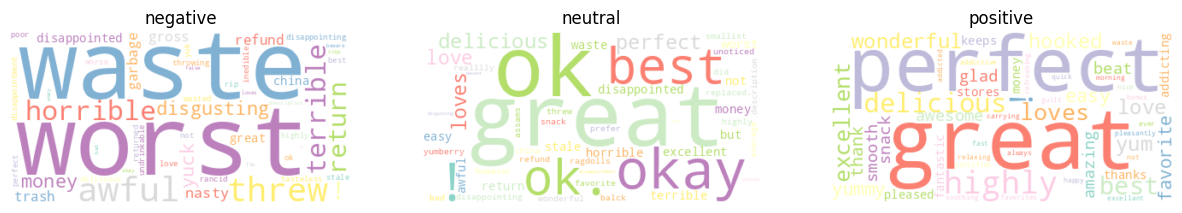
\includegraphics[width=0.78\textwidth]{images/wordcloud_amazon.png}
        \caption{Experiment 1.}
        \label{fig:wordcloud_amazon}
    \end{subfigure}
    
    \bigskip
    
    \begin{subfigure}{\textwidth}
        \centering
        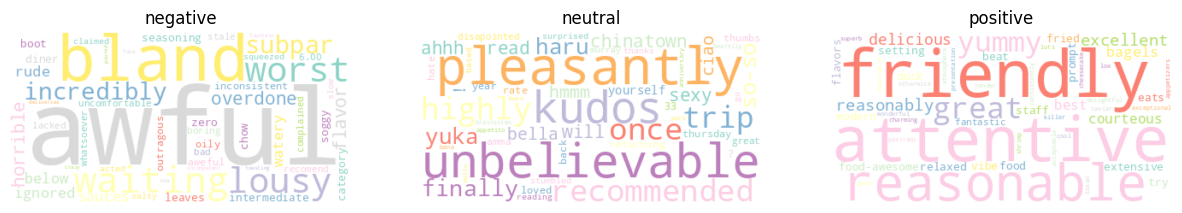
\includegraphics[width=0.78\textwidth]{images/wordcloud_semeval.png}
        \caption{Experiment 2.}
        \label{fig:wordcloud_semeval}
    \end{subfigure}
    
    \bigskip
    
    \begin{subfigure}{\textwidth}
        \centering
        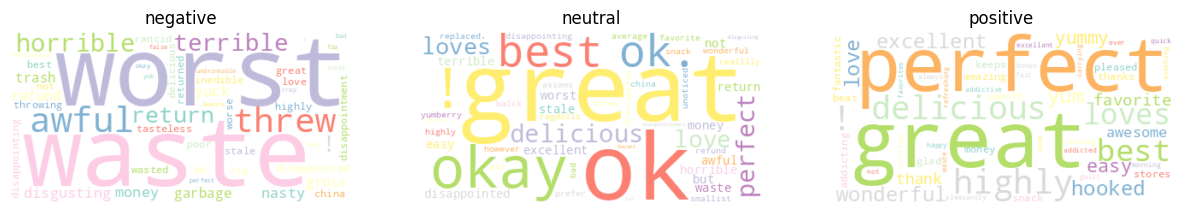
\includegraphics[width=0.78\textwidth]{images/wordcloud_joint.png}
        \caption{Experiment 3.}
        \label{fig:wordcloud_joint}
    \end{subfigure}
    
    \caption{Word clouds of global explanatory features extracted from \texttt{BornClassifier}}
    \label{fig:wordclouds}
\end{figure}

An interesting outcome of the \texttt{BornClassifier} is the global explanatory features, which can be extracted for each of the sentiments. To analyze better, Fig~\ref{fig:wordclouds} represents a word cloud for each of the experiments, visualizing the words according to their weight probability in the global explanations.


% ===========================================
\subsection{Aspect-Based Sentiment Analysis}

This section of the project encompasses the aspect detection and aspect-to-sentence association, each of which is elaborated upon in the following sub-sections:

% ------------------------------------------- 
\subsubsection{Aspect Detection}\label{sec:aspect_detection}

As using the \texttt{AmazonReviewsDataset} for the training set of the sentiment classification was not shown to be effective in detecting the overall sentiment of documents in \texttt{SemEval2014Dataset}, we will proceed to use the model trained on \texttt{SemEval2014Dataset} for our ABSA task.

The \texttt{AspectDetection} class has been designed to encompass all the essential features for the aspect-based sentiment analysis. The strategy for detecting the aspects can be summarized as below:

\begin{enumerate}
    \item \textbf{Acquiring the candidate aspects:} For a given vectorized document, first we predict its overall sentiment, based on which we retrieve the corresponding local explanatory features from the \texttt{BornClassifier}. Then, we keep the non-zero features in the local explanation, which convey the importance of each token of that document in predicting the overall sentiment.

    \item \textbf{Detecting the aspects:} To identify aspects, we filtered the candidate aspect token set, retaining only noun groups as potential aspects. Initially, part-of-speech tagging was performed using the \texttt{pos\_tag} module from \texttt{NLTK}, but its results were unsatisfactory. Therefore, \texttt{spaCy} was employed to obtain more accurate tags.

    \item \textbf{Finalizing the aspect set:} Not all nouns in a document form aspects, so weights from Born's local explanatory features must be analyzed to identify the most informative candidates. Since documents may lack aspects and the exact number of aspects is unknown, selecting the top-\textit{k} features by importance is impractical. Instead, a more sophisticated \texttt{aspect\_threshold} is defined to filter candidates, retaining only those exceeding the specified importance level.

    \item \textbf{Deciding the \texttt{best\_aspect\_threshold}:} Rather than randomly assigning the threshold, NumPy's \texttt{np.linspace} was used to generate \texttt{1200} values within the range \texttt{[0.0001, 0.002]}, each evaluated separately on the training set to determine the optimal threshold for aspect detection, which is then applied to the test set for further evaluation. This optimization alone took \texttt{06:25:11} to complete, giving the corresponding \texttt{best\_aspect\_threshold} of \texttt{0.000395} with F1-score of \texttt{0.568} on the training set. Figure~\ref{fig:threshold_optimization} illustrates this selection process.
\end{enumerate}

\begin{figure}[h]
\centering
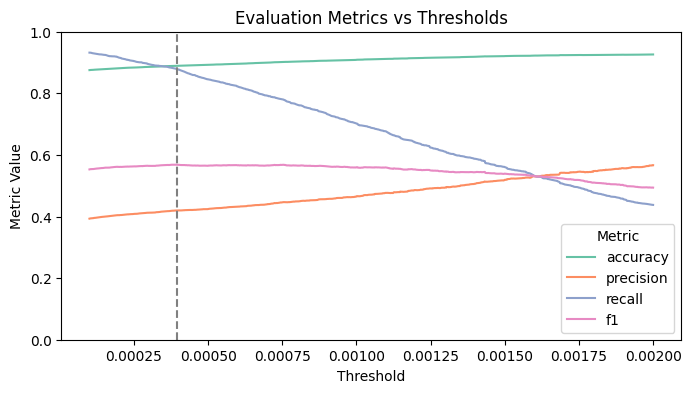
\includegraphics[width=0.9\textwidth]{images/threshold_optimization.png}
\caption{Evaluation metrics for threshold optimization.}\label{fig:threshold_optimization}
\end{figure}

% ------------------------------------------- 
\subsubsection{Aspect-to-Sentence Association}\label{sec:aspect_to_sent}

The \texttt{AspectDetection} class was extended with additional functions to locate the corresponding text portion for each of the aspects. This process can be divided into the following sub-tasks:

\begin{enumerate}
    \item \textbf{Document Segmentation:} The first step involves splitting each document into its composing sentences. Initially, NLTK's \texttt{sent\_tokenize} was used but proved ineffective since most documents in the dataset are short, and sentences are only split when a period (\texttt{.}) is encountered, leaving many unaffected. To improve segmentation, a custom regular expression (\texttt{(?<=[:;.!?()])}) was implemented, yielding significantly better results for the dataset.

    \item \textbf{Aspect Lookup:} To identify the text segment containing a given aspect from those segmented in the previous step, two approaches were evaluated, with the second chosen as the final method:
    
    \begin{itemize}
        \item \textbf{Vectorized Approach:} The candidate aspect tokens derived from Born's explanatory features may have undergone transformations (lowercasing, lemmatization, n-grams), altering their form, hence making it infeasible to perform simple matching. Instead, the token indices for both the aspect and the sentence were identified and checked to see if the aspect's indices were a subset of those in the sentence. However, out-of-vocabulary tokens in the test set, lacking corresponding indices, caused disruptions, making the method unreliable for consistent use.

        \item \textbf{Normal Approach:} Since the only transformation applied to the tokens was lowercasing, it was reasonable to directly search for them within each sentence. Therefore, the first occurrence of a given aspect in any of the segmented text portions was returned as a match.
    \end{itemize}
\end{enumerate}

As an example, given the document \textit{``You must try Odessa stew or Rabbit stew; salads-all good; and kompot is soo refreshing during the hot summer day (they make it the way my mom does, reminds me of home a lot).''} as input with \texttt{['Odessa stew', 'Rabbit stew', 'salads', 'kompot']} as true aspects, Table~\ref{tab:aspect_to_sentence} illustrates the corresponding detected sentence for each of the aspects.

\begin{table}[h]
\caption{Association of Aspects to Text Portions (sentences)}\label{tab:aspect_to_sentence}%
\begin{tabular*}{\textwidth}{@{\extracolsep{\fill}}lll}
\toprule
Aspect & Sentence & Aspect Sentiment \\
\midrule
Odessa stew & You must try Odessa stew or Rabbit stew & Positive \\
Rabbit stew & You must try Odessa stew or Rabbit stew & Positive \\
Salads & salads-all good & Positive \\
Kompot & and kompot is soo refreshing during the hot summer & Positive \\
\botrule
\end{tabular*}
\end{table}